% ================================ LE MODALITÀ DI AES ===================================

\chapter{Le modalità di AES}

% =======================================================================================

% ---------------------------- SECTION: INTRODUZIONE ------------------------------------

\section{Introduzione}

\index{modalità}

\textsf{\small In questa parte tratteremo le varie modalità di crittografia disponibili per AES. Queste ci permetteranno di cifrare messaggi di varia lunghezza.} %TODO: capitolo/In questa parte; su/per AES.

% -------------------------- SECTION: IV, NONCE, SALT E PEPPER --------------------------

\section{IV, Nonce, Salt e Pepper} %TODO: IV, Nonce, Sale e Pepe?

\index{iv} \index{nonce} \index{salt} \index{pepper}

\textsf{\small Prima di poter trattare le modalità è necessario introdurre alcuni componenti che ci serviranno nell'utilizzo di queste. Questi sono l'IV, il nonce, il sale e il pepe.} %TODO: componenti/elementi

\subsection{Nonce | Number Used Once}

\index{nonce}

\textsf{\small Il nonce, \emph{\textbf{n}umber used \textbf{once}} (numero utilizzato una volta), sono dei bits (ovvero un numero) che vengono utilizzati una singola volta. Il riutilizzo non è proibito, ma deve essere limitato.}

\begin{figure}[H]
	\centering
	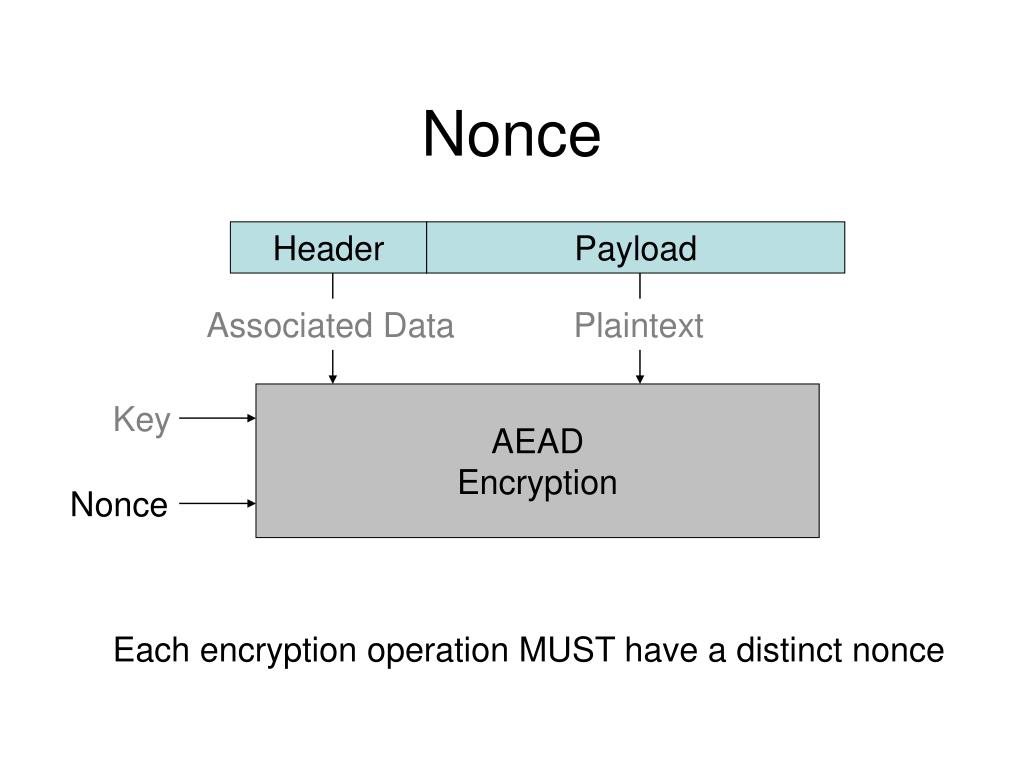
\includegraphics[width=.9\textwidth, height=.9\textheight, keepaspectratio]{./images/iv_nonce_salt_pepper/nonce.png}
	\caption{Nonce}
	\label{fig:nonce}
\end{figure}

\textsf{\small Viene utilizzato nei protocolli di autenticazione per garantire la sicurezza nelle comunicazioni (private) (ed evitare replay attacks).} %TODO:  [da spiegare in un altro capitolo (e aggiungere la \ref alla pagina volendo)

\subsubsection{Nonce sequenziali}

\index{nonce} \index{nonce sequenziali}

\textsf{\small Garantiscono la non ripetizione, se molto grandi.} %TODO: Prevenisco/Garantiscono

%TODO: subsubsection Nonce random?

\subsection{IV | Initialization Vector}

\index{IV}

%TODO: È simile al nonce, ma deve essere casuale/random. Quindi i nonce sequenziali non andrebbero bene.

\textsf{\small L'initialization vector o anche definito starting variables è un input di dimensione fissa, ovvero un numero arbitrario che viene adoperato per impostare lo stato iniziale di un algoritmo crittografico. Viene utilizzato in varie modalità di cifratura per \emph{randomizzare} la cifratura in modo da produrre diversi testi cifrati anche se lo stesso testo viene cifrato molteplici volte.} %TODO: definito/chiamato; fornito/adoperato; produrre/generare

%\subsection{IV vs Nonce} %TODO: forse questa non serve. remove/uncomment?

%\textsf{\small }

\subsection{Salt}

\index{salt} \index{password}

\textsf{\small  Il sale viene utilizzato nelle password per incrementarne la sicurezza. Vengono aggiunti dei caratteri unici casuali alla password, in questo modo un attaccante non necessita solamente di un dizionario di password comuni, ma anche di uno per ogni tipo di sale possibile.} %TODO: salt/sale/password salting

\begin{figure}[H]
	\centering
	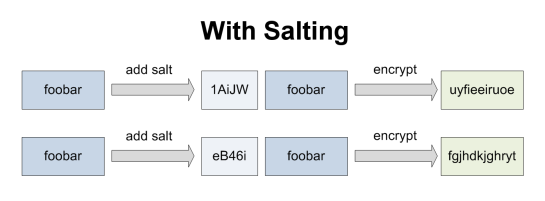
\includegraphics[width=1\textwidth, height=1\textheight, keepaspectratio]{./images/iv_nonce_salt_pepper/withsalting.png}
	\caption{Salt}
	\label{fig:salt}
\end{figure}

\index{database} \index{password}

\textsf{\small Questa tecnica è molto importante e viene utilizzata nei database affinché le password degli utenti siano sicure. (e non possano essere rubate).} %TODO: processo/tecnica

\index{password} \index{salt}

\textsf{\small Le password non vengono mai, possibilmente, memorizzate nei database in chiaro, ma gli viene aggiunto il salt e poi viene eseguito l'hashing su esse.}

\subsection{Pepper}

\index{pepper} \index{salt} \index{password}

\textsf{\small Il pepper è simile al salt, ma questo a differenza del sale che è meramente unico più che segreto, è un (singolo) carattere segreto aggiunto alla fine della password.} %TODO: pepper/pepe; salt/sale; appena/meramente; appeso/aggiunto

\index{hash} \index{password}

\textsf{\small Questo, (a differenza del sale) non viene memorizzato nello stesso database assieme alla password hash e al sale, ma a parte.}

% ---------------------------- SECTION: IL PADDING --------------------------------------

\section{Il padding}

\index{padding}

\textsf{\small Un altro elemento utilizzato nei cifrari a blocchi è il padding. }
\textsf{\small Il padding serve per riempire i blocchi del cifrario con dei bytes.}

\index{padding oracle attack}

\textsf{\small È un modo per cifrare messaggi anche di grandezze che il cifrario non sarebbe in grado di decifrare.}
\textsf{\small Non aumenta la sicurezza, anzi se mal implementato può portare ad attacchi di padding (\emph{padding oracle attack}).} %TODO: portare/causare. %TODO: approfondire magari anche con \ref nel capitolo sugli attacchi.

\textsf{\small Grazie a questa tecnica, è possibile aggiungere, all'inizio, al centro o in fondo al messaggio, del nonsense per oscurare parti del messaggio che altrimenti sarebbero prevedibili, come: \emph{Caro...}, \emph{Gentile...}, \emph{Cordiali Saluti..}, ecc.}

\textsf{\small I principali meccanismi di padding sono: }

\index{padding} \index{no padding} \index{0-Padding} \index{1-0-Padding} \index{ANSI X9.23 Padding} \index{ISO 10126 Padding} \index{PKCS7}

%TODO: uncomment, magari mostrare degli esempi per ognuno di questi?
\begin{itemize}
	\item \textsf{\small \textbf{No padding}: Nessun padding viene aggiunto al messaggio.}
	\item \textsf{\small \textbf{0-Padding}: Vengono aggiunti dei bytes con degli zeri alla fine dell'ultimo blocco, finché non abbiamo il corretto numero di bytes (in AES è 16 bytes); se già abbiamo il numero necessario di bytes, allora non viene aggiunto nulla}
	\item \textsf{\small \textbf{1-0-Padding}: Viene aggiunto un byte a 1 e il restante viene riempito da bytes di 0 finché non abbiamo il numero necessario di bytes; se il numero di bytes necessario è già presente, allora aggiungiamo un altro blocco.}
	\item \textsf{\small \textbf{ANSI X9.23 Padding}: Aggiungiamo bytes di 0 alla fine dell'ultimo blocco, finché non abbiamo 16 - 1 bytes. Nell'ultimo blocco inseriamo il numero totale di bytes a 0 che abbiamo aggiunto; se l'ultimo blocco è già pieno (corrisponde a 16 bytes), allora aggiungiamo blocco addizionale.}
	\item \textsf{\small \textbf{ISO 10126 Padding}: Vengono aggiunti dei bytes casuali in fondo all'ultimo blocco, finché non abbiamo 16 - 1 bytes e nell'ultimo byte inseriamo il numero totale di bytes casuali che abbiamo immesso; Se l'ultimo blocco è già 16 bytes, allora aggiungiamo un altro blocco.}
	\item \textsf{\small \textbf{PKCS\#7}: Aggiungiamo il numero totale di bytes che restano per riempire il blocco in ogni byte rimanente, finché non abbiamo 16 bytes.}
	%\item \textsf{\small }
	%\item \textsf{\small }
\end{itemize}

% ---------------------------- SECTION: PERCHÉ SERVE UNA/LE MODALITÀ? PERCHÉ USARE UNA/LE MODALITÀ? A COSA SERVONO LE MODALITÀ? ------------

\section{A cosa servono le modalità?}

\index{modalità} \index{AES} \index{blocco} \index{chiave}

\textsf{\small Le modalità servono, perché AES è un cifrario a blocchi di 16 bytes, dopo aver preso un blocco e una chiave in input restituisce un altro blocco della medesima grandezza.} %TODO: grandezza/lunghezza

\index{modalità di cifratura}

\textsf{\small Quindi, se si desidera cifrare una sequenza di bytes di lunghezza maggiore di 16, è necessario utilizzare una \emph{modalità di operazione} o \emph{modalità di cifratura}.} %TODO: 16 bytes; lunghezza/grandezza; desidera/vuole; bisogna/è

\index{modalità}

\textsf{\small Queste modalità sono indipendenti dal tipo di cifrario che sta alla base.} %TODO: sottostante/che sta alla base

\begin{figure}[H]
	\centering
	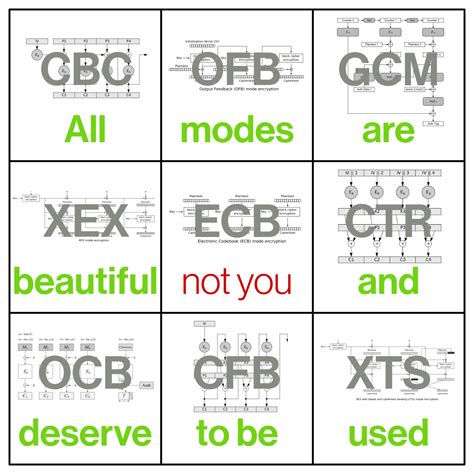
\includegraphics[width=.8\textwidth, height=.8\textheight, keepaspectratio]{./images/aes_modes/modes.png} % prima aes_modes.png
	\caption{Modalità di AES}
	\label{fig:aes_modes}
\end{figure}

% ---------------------------- SECTION: LE MODALITÀ -------------------------------------

\section{Le modalità}

\index{modalità} \index{modalità di cifratura}

\textsf{\small Qui, di seguito elencherò le caratteristiche e proprietà delle principali modalità di cifratura:}

\subsection{Modalità di cifratura senza integrità del messaggio}

\index{modalità} \index{modalità di cifratura} \index{modalità di cifratura senza integrità del messaggio}

\begin{figure}[H]
	\centering
	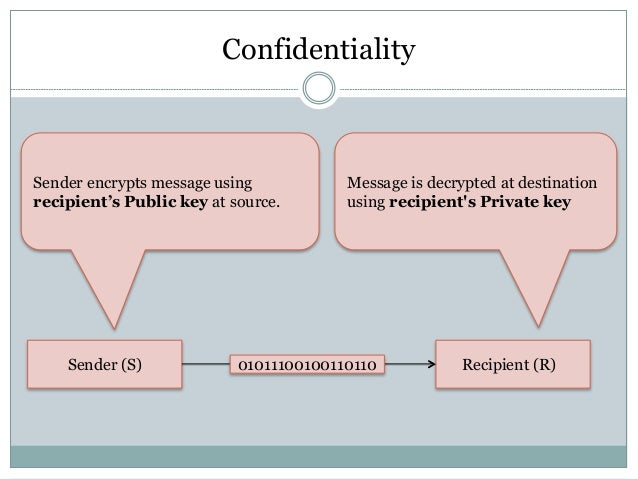
\includegraphics[width=.9\textwidth, height=.9\textheight, keepaspectratio]{./images/aes_modes/confidentiality.png}
	\caption{Confidenzialità}
	\label{fig:confidentiality}
\end{figure}

\index{modalità} \index{messaggio}

\textsf{\small Queste modalità forniscono la cifratura del messaggio, ma non garantisco l'integrità del messaggio, ovvero non è assicurato che il messaggio non sia stato manomesso e quindi non è possibile accertare l'autenticazione del messaggio originale.} %TODO: ovvero/quindi; manomesso/alterato %TODO: magari riguardare la parte dell'"accertare l'autenticazione del messaggio originale"

\subsubsection{ECB | Electronic Code Book}

\index{modalità} \index{ECB} \index{blocchi}

\textsf{\small Questa modalità di cifratura divide il nostro messaggio in diversi blocchi e ognuno di questi viene cifrato separatamente.}

\index{modalità}

\textsf{\small Questa modalità manca il principio di diffusione e quindi cifra lo stesso messaggio in chiaro nello stesso testo cifrato, quindi non vela il pattern dei dati.} %TODO: (aggiungere \ref a diffusione); dei dati/i dati

\index{ECB} \index{modalità}

\textsf{\small In generale, ECB è considerata una modalità obsoleta, da non utilizzare. È una modalità molto debole e poco sicura.}

\begin{figure}[H]
	\centering
	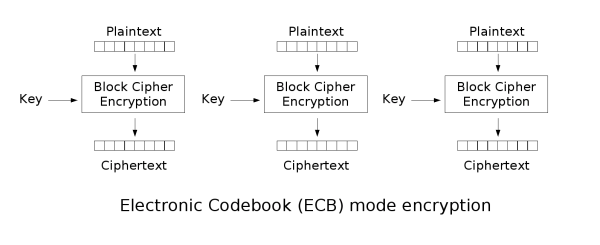
\includegraphics[width=.9\textwidth, height=.9\textheight, keepaspectratio]{./images/aes_modes/ecb_encryption.png} % mettere 1 e 1?
	\caption{ECB}
	\label{fig:ecb}
\end{figure}

\textsf{\small Come si deduce dall'immagine, ogni blocco viene cifrato indipendentemente. Viene inserito il messaggio in chiaro e la chiave all'interno del cifrario per ottenere il testo cifrato. Blocchi di testo in chiaro uguali vengono cifrati allo stesso modo.}

\textsf{\small Per questo, osservando il testo cifrato è possibile riconoscere, se presenti nel testo in chiaro, parti cifrate allo stesso modo. }

\textsf{\small Per decifrare, eseguiamo l'operazione inversa, immettendo un blocco cifrato assieme alla chiave, per ottenere il testo decifrato.}

\index{ECB}

\textsf{\small Ricapitolando i problemi di ECB:}

\begin{itemize}
	\item \textsf{\small ECB è deprecato e non dovrebbe essere utilizzato.}
	\item \textsf{\small Gli stessi blocchi di messaggio vengono cifrati con gli stessi blocchi cifrati.}
\end{itemize}

%TODO: Aggiungere immagine/schema della decifrazione?

\subsubsection{CBC | Cipher Block Chain}

\index{CBC} \index{ECB} \index{IV} \index{XOR}

\textsf{\small La modalità CBC cerca di ovviare ai problemi dell'ECB aggiungendo della casualità a ogni operazione di cifratura usufruendo di un initialization vector (IV) per il primo blocco e dopodiché applicando uno XOR a ogni blocco di testo in chiaro con il blocco cifrato precedente.} %TODO: precedente/precedentemente

\begin{figure}[H]
	\centering
	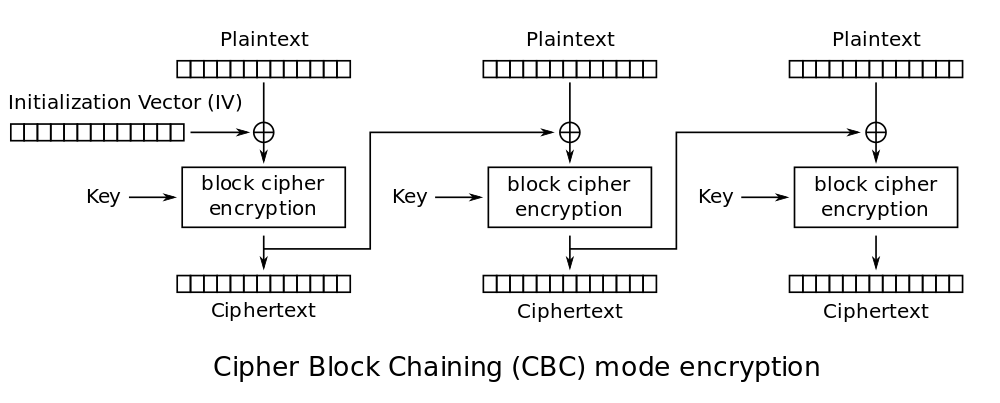
\includegraphics[width=1\textwidth, height=1\textheight, keepaspectratio]{./images/aes_modes/cbc.png} % mettere 1 e 1?
	\caption{CBC}
	\label{fig:cbc}
\end{figure}

\textsf{\small Ricapitolando le fasi che si evincono dallo shema, qui sopra:}

\index{IV} \index{XOR} \index{ECB}

\begin{itemize}
	\item \textsf{\small Collega ("Incatena" da \emph{Chaining}) tutti i blocchi.}
	\item \textsf{\small L'IV (\emph{\textbf{I}nitialization \textbf{V}ector}) è usato per modificare il testo in chiaro.}
	\item \textsf{\small Viene eseguito lo XOR tra il blocco cifrato precedente e il blocco col testo in chiaro corrente.}
	\item \textsf{\small Risolve il problema dei blocchi di testo in chiaro uguali che vengano cifrati allo stesso modo. (problema presente in ECB)}
	\item \textsf{\small Modificando un bit di un blocco di testo in chiaro, modifica di conseguenza tutti gli altri blocchi cifrati a seguire.}
\end{itemize}

%TODO: Aggiungere immagine/schema della decifrazione?

\index{CBC}

\textsf{\small Sono possibili degli attacchi su CBC, se l'attaccante modifica ogni secondo blocco in chiaro se è a conoscenza dell'intero testo in chiaro.}

\index{IV} \index{nonce} \index{nonce semplice}

\textsf{\small Questa modalità è sicura come uno schema probabilistico e la confidenzialità non viene raggiunta se l'IV è un nonce semplice.} %TODO: forse approfondire cos'è un nonce semplice

\subsubsection{CFB | Cipher Feedback}

\index{CFB} \index{CBC} \index{stream} \index{a blocchi}

\textsf{\small CFB è molto simile a CBC, ma al posto di essere un cifrario a blocchi, è un cifrario a stream, \emph{stream cipher}, ovvero un cifrario che prende una chiave e un algoritmo e lo applica allo stream (un bit alla volta), a ogni singolo bit (bit a bit) e non a blocchi di bits.}

\begin{figure}[H]
	\centering
	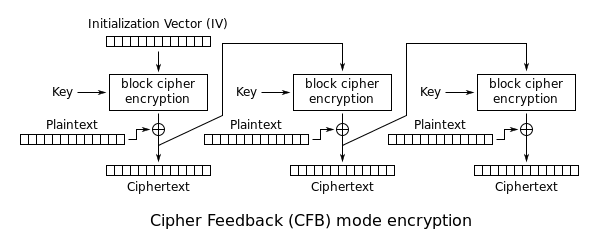
\includegraphics[width=1\textwidth, height=1\textheight, keepaspectratio]{./images/aes_modes/cfb.png}
	\caption{CFB}
	\label{fig:cfb}
\end{figure}

\textsf{\small Ricapitolando lo schema presente qui sopra:}

\index{CBC} \index{XOR} \index{stream cipher} \index{cifrario a flusso}

\begin{itemize}
	\item \textsf{\small Lega tutti i blocchi (proprio come CBC).}
	\item \textsf{\small Genera dei bytes casuali che vengono poi successivamente "XORati" col blocco di testo in chiaro.}
	\item \textsf{\small Trasforma il cifrario a blocchi in uno stream cipher (cifrario a flusso).}
\end{itemize}

%TODO: Aggiungere immagine/schema della decifrazione?

\subsubsection{OFB | Output Feedback}

\index{OFB}

\begin{figure}[H]
	\centering
	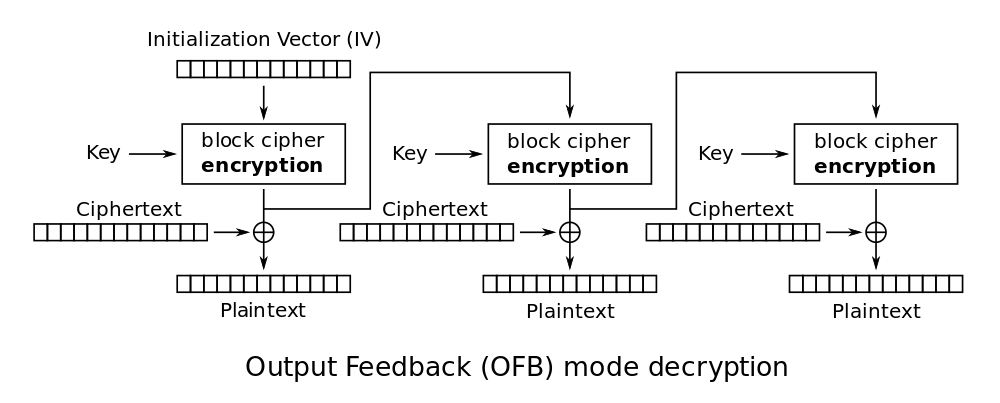
\includegraphics[width=1\textwidth, height=1\textheight, keepaspectratio]{./images/aes_modes/ofb.png} % mettere 1 e 1?
	\caption{OFB}
	\label{fig:ofb}
\end{figure}

\index{stream cipher} \index{iv} \index{XOR}

\textsf{\small È anch'esso un \emph{stream cipher}, cifra l'iv (genera una serie di caratteri casuali)  e poi esegue uno XOR per ottenere il testo cifrato.}

\textsf{\small Ogni operazione dipende da quelle precedenti.}

\index{OFB} \index{CFB}

\textsf{\small Ricapitolando le operazioni dell'OFB, proprio come il CFB:}

\index{CBC} \index{CFB} \index{XOR} \index{stream cipher} \index{cifrario a flusso}

\begin{itemize}
	\item \textsf{\small Lega tutti i blocchi (proprio come CBC e CFB).}
	\item \textsf{\small Genera dei bytes casuali, un flusso usando il cifrario che viene poi successivamente XOR col blocco di testo in chiaro.}
	\item \textsf{\small Trasforma il cifrario a blocchi in uno stream cipher (cifrario a flusso).}
\end{itemize}

\index{CFB} \index{IV}

\textsf{\small L'unica differenza con CFB è che al posto di utilizzare il testo cifrato nei blocchi successivi, utilizza l'output dei bytes casuali generati dal cifrario attraverso la chiave e l'IV per il blocco successivo.}

\subsubsection{CTR | Counter Mode}

\index{CTR} \index{IV}

\textsf{\small La Counter Mode o CM (\emph{integer counter mode}) o SIC (\emph{segmented integer counter}) usufruisce di un counter (contatore), ovvero di una funzione che genera sequenze irripetibili (nel tempo), al posto di utilizzare un IV.}

\textsf{\small Il più semplice contatore è il banale incrementa di 1.}
\textsf{\small Questa modalità può essere parallelizzata.}

\begin{figure}[H]
	\centering
	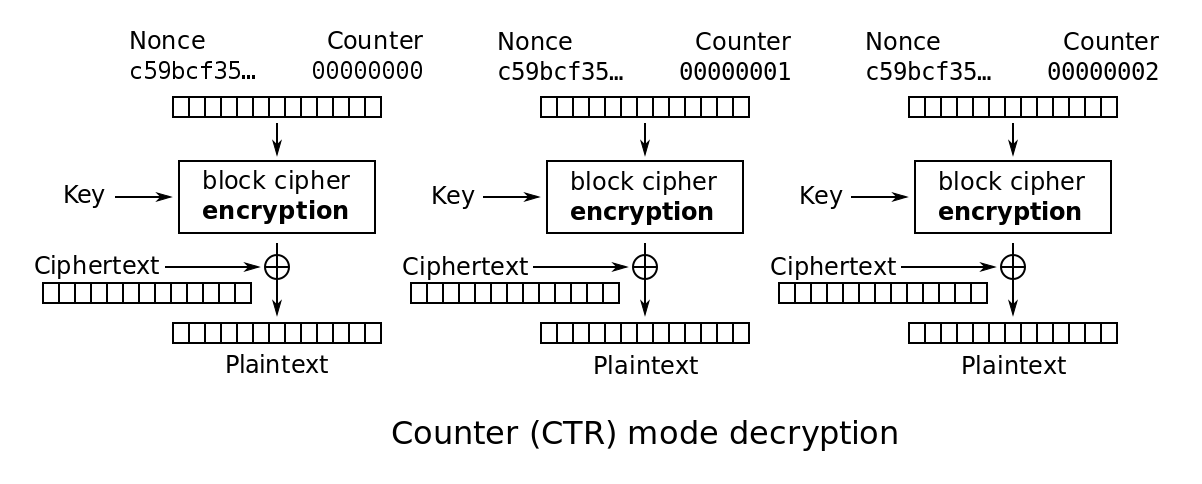
\includegraphics[width=1\textwidth, height=1\textheight, keepaspectratio]{./images/aes_modes/ctr.png}
	\caption{CTR}
	\label{fig:ctr}
\end{figure}

\subsubsection{XTS | AES-XTS (XEX) Tweakable Block Cipher}

\index{XTS} \index{AES}

\textsf{\small Questa modalità è utilizzata per cifrare/decifrare i dischi rigidi (hard-disk), quindi la cifratura verrà operata sui segmenti da 512 bytes (ovvero 32 blocchi di AES-128) e i rispettivi settori (del disco).}

\index{modalità}

\textsf{\small Questa modalità compie le seguenti operazioni: } %TODO: Questa modalità esegue/è composta/compie/effettua le seguenti operazioni:

\index{XOR} \index{AES}

\begin{itemize}
	\item \textsf{\small Definite due chiavi: K1, K2 (utilizzando AES-128), Blocco di input, p, numero settore, \emph{i} e un numero del blocco, \emph{j}, definiamo il "tweak", \emph{X}, nel seguente modo:}
	\begin{itemize}
		\item \textsf{\small $X = E_{K_2}(i) \otimes 2^j$}
	\end{itemize}
	\item \textsf{\small Di conseguenza, il testo cifrato C è definito così:}
	\begin{itemize}
		\item \textsf{\small $C = P \oplus X$}
		\item \textsf{\small ovvero testo cifrato = blocco di input "XORato" con il tweak.}
		\item \textsf{\small $C = E_{K_1}(C) \oplus X$}
	\end{itemize}
	\item \textsf{\small Per poter decriptare, invece, eseguiamo: }
	\begin{itemize}
		\item \textsf{\small $X = E_{K_2} (i) \otimes 2^j$}
	\end{itemize}
	\item \textsf{\small il testo in chiaro, per ogni blocco, è:}
	\begin{itemize}
		\item \textsf{\small $P = C \oplus X$}
		\item \textsf{\small $P = E^{-1}_{K_1} (P) \oplus X$}
	\end{itemize}
	\item \textsf{\small In questo modo, il tweak fa da IV.}
	%\item \textsf{\small }
\end{itemize}

\textsf{\small }

\begin{figure}[H]
	\centering
	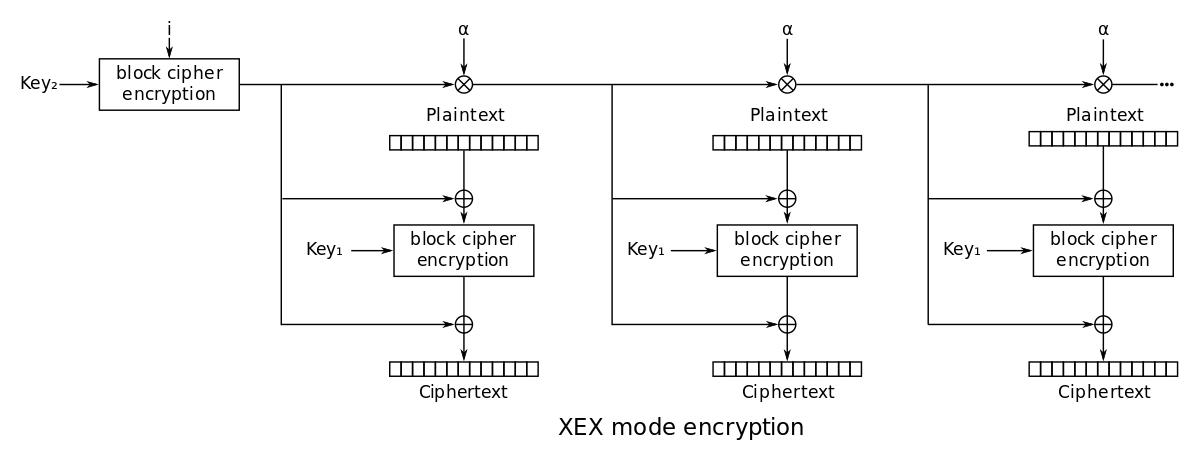
\includegraphics[width=1\textwidth, height=1\textheight, keepaspectratio]{./images/aes_modes/xex.png}
	\caption{XEX}
	\label{fig:xex}
\end{figure}

%TODO: subsection EAX | encrypt-then-authenticate-then-translate. metterlo o no?

\subsection{MACS | Message Authentication Codes}

\index{MACS} \index{MAC}

\textsf{\small I MACS permettono di verificare l'integrità del messaggio per potersi assicurare che non sia stato alterato da parti esterne e che il messaggio giunga integro ai destinatari originali.} %TODO: manomesso/alterato; arrivi/giunga; intero/integro

\begin{figure}[H]
	\centering
	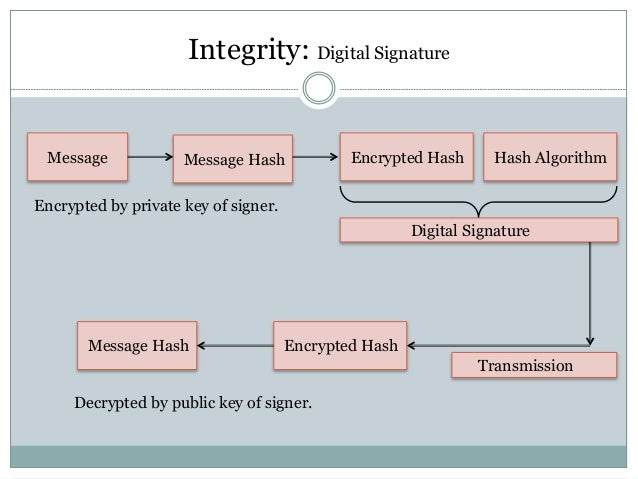
\includegraphics[width=.9\textwidth, height=.9\textheight, keepaspectratio]{./images/aes_modes/encryption-integrity-and-nonrepudiation.png}
	\caption{Integrità e non ripudio}
	\label{fig:encryption-integrity-and-nonrepudiation}
\end{figure}

\index{MACS}

\textsf{\small Quindi, i MACS formano una tipologia di firma digitale dove tutte le parti considerate possono verificare che i dati ricevuti siano validi.}

\textsf{\small Questo grazie a un meccanismo a 3 componenti:}

\begin{enumerate}
	\item \textsf{\small Chiave segreta: chiave segreta condivisa dalle parti.}
	\item \textsf{\small MAC Signing Algorithm: si avvale della chiave e del messaggio per generare un tag (\emph{authentication tag}) che permette di verificare che i dati siano integri e non truccati)}
	\item \textsf{\small MAC Validation Algorithm: prende in input la chiave, il messaggio, il tag e restituisce in output la validità del tag, ovvero se il messaggio è stato violato, modificato o no.}
\end{enumerate}

\subsubsection{ALG1-6}

\index{ALG1-6} \index{MACS} \index{MAC} \index{CBC-MAC}

\textsf{\small È una collezione di MACs basati su CBC-MAC, di cui alcuni sicuri come il VIL PRF, FIL PRF altri non ne abbiamo certezza.}

\subsubsection{CMAC | Cipher-based Message Authentication Code}

\index{CMAC} \index{MAC}

\textsf{\small CMAC è una modalità basata su CBC-MAC. Questa crea un messaggio di autenticazione (MAC) utilizzando un cifrario a blocchi e una chiave segreta. }

\begin{figure}[H]
	\centering
	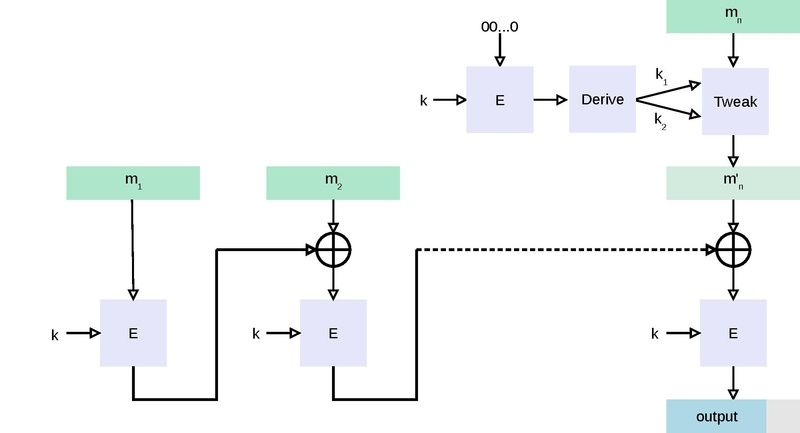
\includegraphics[width=.9\textwidth, height=.9\textheight, keepaspectratio]{./images/aes_modes/CMAC_-_Cipher-based_Message_Authentication_Code}
	\caption{CMAC}
	\label{fig:cmac}
\end{figure}

\subsubsection{HMAC | Keyed-hash Message Authentication Code}

\index{HMAC} \index{MAC} \index{hashing} \index{hash} \index{MD5} \index{SHA-1} \index{SHA-256} \index{SHA-2} \index{SHA-3}

\textsf{\small HMAC è una modalità che permette di autenticare gli emittenti del messaggio attraverso autenticazione basata su algoritmi di hashing, come: MD5, SHA-1, SHA-256 (SHA-2) e SHA-3.}

\textsf{\small La sicurezza di questa modalità è stata provata.}

\subsubsection{GMAC | Galois Message Authentication Code}

\index{GMAC} \index{Galois}

\textsf{\small Questa modalità è una specializzazione della modalità \textbf{GCM} (\emph{\textbf{G}alois/\textbf{C}ounter \textbf{M}ode}). Viene utilizzata per l'autenticazione.}

\begin{figure}[H]
	\centering
	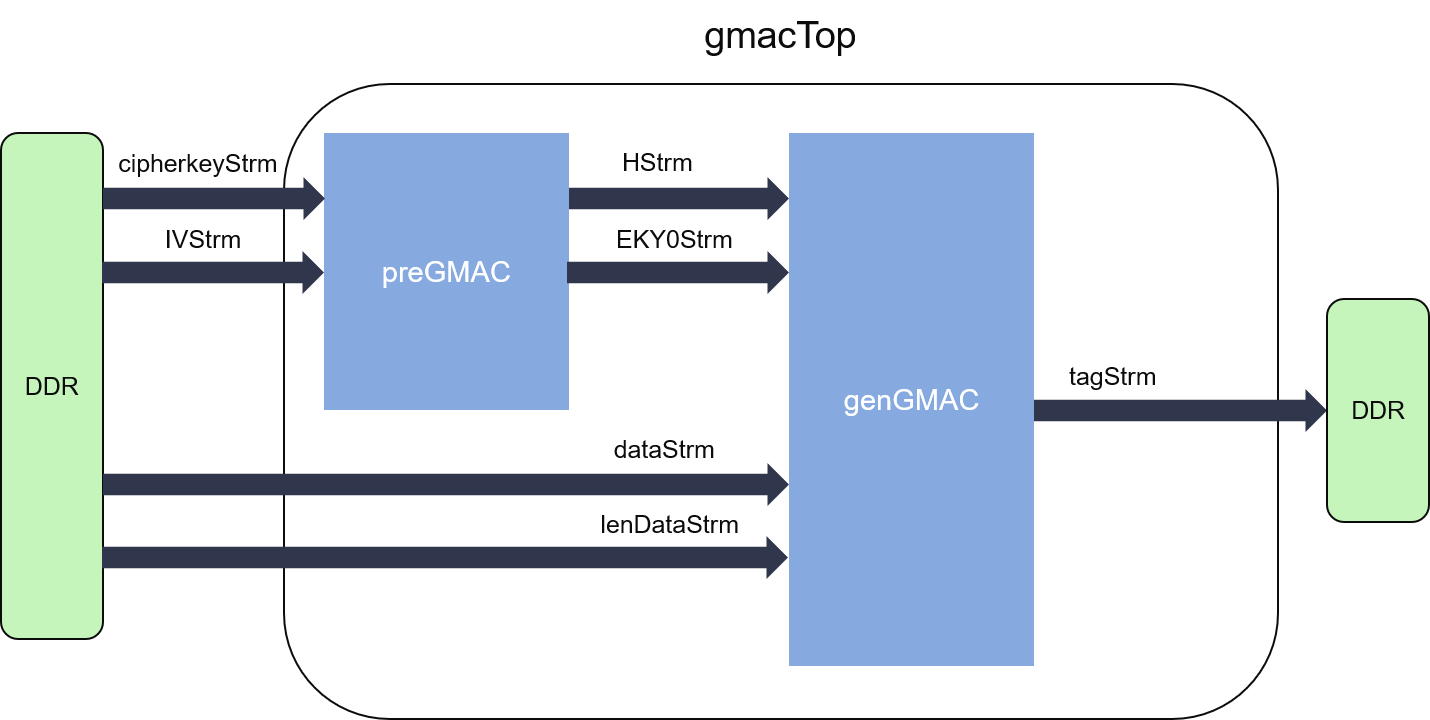
\includegraphics[width=.9\textwidth, height=.9\textheight, keepaspectratio]{./images/aes_modes/internal_structure_of_gmac} %TODO: gcm
	\caption{GMAC}
	\label{fig:gmac}
\end{figure}

\subsubsection{CBC-MAC}

\index{CBC-MAC} \index{MAC} \index{CBC}

\textsf{\small CBC-MAC combina la modalità CBC (Cipher Block Chaning) assieme al MAC per l'autenticazione dei mittenti del messaggio.}

\begin{figure}[H]
	\centering
	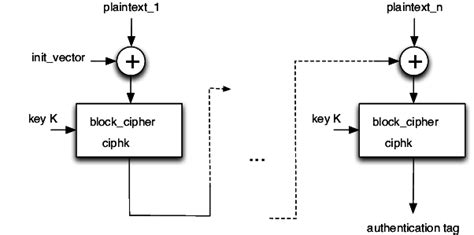
\includegraphics[width=.9\textwidth, height=.9\textheight, keepaspectratio]{./images/aes_modes/cbc-mac}
	\caption{CBC-MAC}
	\label{fig:cbc-mac}
\end{figure}

\subsection{AEAD | Authenticated Encryption with Associated Data}

\index{AEAD}

\textsf{\small AEAD è un modello di cifratura che assicura sia la riservatezza del messaggio sia la sua autenticazione.}

\subsubsection{OCB | Offset Codebook} %TODO: section MACS? AEAD

%TODO: Aggiungere qualcos'altro su questa modalità.

\index{OCB}

\textsf{\small Questa modalità è stata ideata da Phillip Rogaway con l'assistenza di Mihir Bellare, John Black e Ted Krovetz, basata sull'IAPM (\emph{\textbf{I}ntegrity-\textbf{A}ware \textbf{P}arallelizeable \textbf{M}ode}) che permette di parallelizzare la modalità.}

\textsf{\small Sono presenti tre versioni di OCB: OCB1, OCB2 e OCB3.}

\index{OCB}

\textsf{\small OCB, rispetto alle altre modalità, è molto più veloce.}

\textsf{\small Erano presenti due brevetti su questa modalità che ne impedivano l'esteso utilizzo, ma dal 2021 questi sono stati abbandonati.} %TODO: utilizzo/la diffusione

\subsubsection{CCM | Counter con CBC-MAC}

\index{CCM} \index{CBC-MAC} \index{nonce} \index{AEAD} \index{CTR}

\textsf{\small CCM è un AEAD basato su Nonce che combina le modalità CTR e CBC-MAC i cui blocchi devono essere composti da 128 bits.}

\subsubsection{GCM | Galois Counter Mode}

\index{GCM} \index{AEAD} \index{CTR} \index{Galois} \index{nonce} \index{MAC} 

\textsf{\small È un AEAD basato su Nonce che combina le modalità CTR per l'operazione di cifratura e il campo di Galois (Galois Field) GF($2^{128}$) per l'autenticazione.}

\index{GMAC} \index{Nonce-MAC}

\textsf{\small Può essere usato come Nonce-MAC, in quel caso viene denominato \textbf{GMAC}.}

\begin{figure}[H]
	\centering
	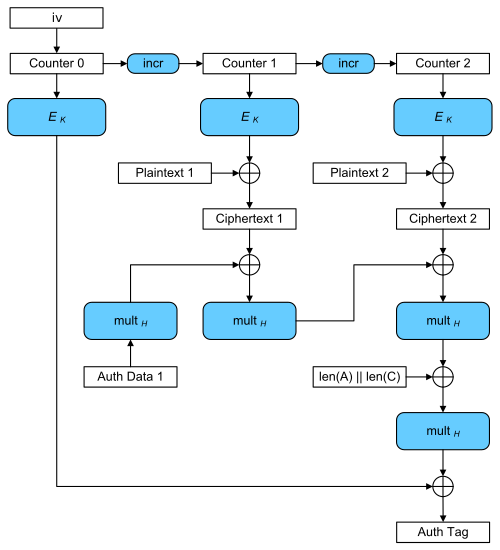
\includegraphics[width=.9\textwidth, height=.9\textheight, keepaspectratio]{./images/aes_modes/GCM-Galois_Counter_Mode_with_IV} 
	\caption{GCM}
	\label{fig:gcm}
\end{figure}

% ================================== FINE CAPITOLO ========================================